% !TeX TXS-program:compile = txs:///pdflatex/[--shell-escape]

\documentclass[11pt, letterpaper]{article}

\usepackage[utf8]{inputenc}
\usepackage{minted}
\usepackage[T1]{fontenc}
\usepackage{lmodern}
\usepackage{graphicx}
\usepackage{longtable}
\usepackage{wrapfig}
\usepackage{rotating}
\usepackage{amsmath}
\usepackage{textcomp}
\usepackage{amssymb}
\usepackage{hyperref}
\usepackage[spanish]{babel}
\usepackage[round]{natbib}
\usepackage{subcaption}

\title{\bfseries Tarea}
\author{Ángel García Báez}
\date{\today}
\setcounter{tocdepth}{4} 

\begin{document}
	
	% Página de presentación
	\begin{titlepage}
		\centering
		
\includegraphics[width=0.2\textwidth]{logo.png}\par
		\vspace{1cm}
		{\LARGE \bfseries Universidad Veracruzana \par}
		\vspace{1cm}
		{\Large Maestría en Inteligencia Artificial\par}
		\vspace{3cm}
		{\LARGE \bfseries Lógica difusa \par}
		\vspace{1cm}
		{\Large \bfseries Tarea 9. Implementación del algoritmo de Fuzzy C-means en MATLAB. \par}
		\vfill
		{\Large \textit{Ángel García Báez}\par}
		\vfill
		{\Large Dr. Sergio Hernández Méndez \par}
		\vfill
		{\Large \today \par}
	\end{titlepage}
	
	% Página exclusiva para la tabla de contenidos
	\newpage
	\tableofcontents
	\newpage
	
% Explicación breve

\section{Introducción}

En el presente reporte se plantea la idea de aplicar el  algoritmo de agrupación con lógica difusa "Fuzzy C-means" para probarlo sobre un conjunto de datos de jugadores de futbol, del cual se tienen 2 variables medidas por cada uno de ellos: rapidez y resistencia.




\newpage

\section{Definiciones}

\subsection{Distancia}

Acorde con \cite{wang_survey_2015}, para un conjunto de datos tal que si $x,y,z \in M$ son vectores de datos de la misma dimensionalidad, se puede definir $D: M\times M \rightarrow R$ como una distancia métrica si se satisfacen las siguientes propiedades:


\begin{itemize}
	\item No negatividad: $D(x,y)$.
	
	\item Coincidencia: $D(x,y) = 0$ si y solo si $x = y$.
	
	\item Simetría: $D(x,y) = D(y,x)$
	
	\item Subaditividad: $D(x,y) + D(y,z) \geq D(x,z)$
	
\end{itemize}

Las siguientes definiciones de distancias se obtuvieron del articulo de revisión de \cite{wang_survey_2015}:


\subsection{Distancia Euclidiana}


$$d(x_1,x_2) = \sqrt{\sum{(x_1-x_2)^2}}$$

Donde:

\begin{itemize}
	\item $x_1$ es el vector fila de tamaño $1\times P$.
	\item $x_2$ es el vector fila de tamaño $1\times P$.
	\item $\sum{(x_1-x_2)^2}$ Es la suma de las diferencias al cuadrado de cada componente de los vectores, el resultado es un escalar. 
\end{itemize}





\subsection{Distancia Mahalanobis}

$$d(x_1,x_2) = \sqrt{(x_1-x_2)\Sigma^{-1}(x_1-x_2)^{T}}$$

Donde:

\begin{itemize}
	\item $x_1$ es el vector fila de tamaño $1\times P$.
	\item $x_2$ es el vector fila de tamaño $1\times P$.
	\item $\Sigma^{-1}$ es la inversa de la matriz de varianzas y covarianzas de todo el conjunto de datos al que pertenecen los vectores. 
\end{itemize}


\subsection{Distancia Manhattan}

$$d(x_1,x_2) = \sum{|(x_1-x_2)|}$$

\begin{itemize}
	\item $x_1$ es el vector fila de tamaño $1\times P$.
	\item $x_2$ es el vector fila de tamaño $1\times P$.
	\item $\sum{(x_1-x_2)^2}$ Es la suma de las diferencias en valor absoluto de las componentes de los vectores, el resultado es un escalar.
\end{itemize}


\newpage

\subsection{Algoritmo para fuzzy c-means}

El algoritmo fuzzy c-means fue propuesto en un inicio por \cite{nascimento_fuzzy_2000} como una alternativa para el agrupamiento de datos en el contexto del aprendizaje no supervisado de tal forma que se le pudiera agregar esta capa de computo suave al proceso con el fin de llegar a mejores resultados.

A continuación se muestra una versión del algoritmo que es explicada de forma más clara y concisa que fue obtenida de 
\cite{edla_analysis_2020}:

\subsubsection{Paso 1}

Inicializa la matriz $U(t)$ (matriz de pertenencias) de tamaño $n\times k$ con valores aleatorios entre 0 y 1, de tal forma que cada fila sume 1.

\subsubsection{Paso 2}

Calcula el valor de los $k$ centroides haciendo uso de la matriz de pertenencias $U(t)$ acorde con la siguiente formula:

$$vk = \frac{\sum^n_{i = 1}{u^m_{ki}xi}}{\sum^n_{i = 1}{u^m_{ki}}}$$

\begin{itemize}
	\item $v_k$: Centroide del cluster $k$ (vector de características promedio ponderado).
	\item $n$: Número total de datos o muestras.
	\item $u_{ki}$: Grado de pertenencia del dato $i$ al cluster $k$.
	\item $m$: Parámetro de difusidad o fuzzificación ($m > 1$).
	\item $x_i$: Vector de características del dato $i$.
	\item $\sum_{i=1}^{n} u_{ki}^m x_i$: Suma ponderada de los datos $x_i$ por el grado de pertenencia elevado a $m$.
	\item $\sum_{i=1}^{n} u_{ki}^m$: Suma de los grados de pertenencia elevados a $m$ (factor de normalización).
\end{itemize}


\subsubsection{Paso 3}

Actualizar la matriz $U(t) $, con la matriz $U(t + 1)$ reemplazando los elementos de la matriz con los siguientes:

$$u_{ki} = \frac{1}{\sum^c_{j = 1}{\frac{||x_i-v_k||}{||x_i-v_j||}}^{2/(m-1)}}$$

\begin{itemize}
	\item $u_{ki}$: Grado de pertenencia del dato $i$ al cluster $k$.
	\item $c$: Número total de clusters.
	\item $j$: Índice que recorre todos los clusters de $1$ a $c$.
	\item $x_i$: Vector de características del dato $i$.
	\item $v_k$: Centroide del cluster $k$.
	\item $v_j$: Centroide del cluster $j$.
	\item $||x_i - v_k||$: Distancia entre el dato $i$ y el centroide $k$.
	\item $||x_i - v_j||$: Distancia entre el dato $i$ y el centroide $j$.
	\item $m$: Parámetro de difusidad o fuzzificación ($m > 1$).
	\item $\sum_{j=1}^{c} \left( \frac{||x_i - v_k||}{||x_i - v_j||} \right)^{2/(m-1)}$: Suma que normaliza las pertenencias relativas del punto $x_i$ respecto a todos los centroides.
\end{itemize}


\subsubsection{Paso 4}

Verificar que $||U(t)-U(t+1)||<\epsilon$, si la diferencia de la anterior con la nueva matriz de pertenencias es menor al limite de tolerancia permitido, detiene el proceso, si no, vuelve al paso 2 y sigue iterando hasta alcanzar un máximo de iteraciones (fijado a 100 para efectos prácticos).


\newpage

\section{Metodología}


La metodología de experimentación propuesta para observar el comportamiento del algoritmo bajo distintas combinaciones de parámetros, es realizar 3 corridas por cada una de las distancias (Euclidiana, Mahalanobis y Manhattan), con $k=3$ grupos, una tolerancia $\epsilon = 0.001$, un máximo de iteraciones de 100  y variando al parámetro $M$ por valores de 1.3, 1.6 y 1.9.

La base de datos para trabajar es la siguiente:


\begin{table}[ht]
	\centering
	\begin{tabular}{cc}
		\hline
		\textbf{Rapidez} & \textbf{Resistencia} \\
		\hline
		0.58 & 0.33 \\
		0.90 & 0.11 \\
		0.68 & 0.17 \\
		0.11 & 0.44 \\
		0.47 & 0.81 \\
		0.24 & 0.83 \\
		0.09 & 0.18 \\
		0.82 & 0.11 \\
		0.65 & 0.50 \\
		0.09 & 0.63 \\
		0.98 & 0.24 \\
		0.90 & 0.33 \\
		0.46 & 0.80 \\
		0.48 & 0.19 \\
		0.03 & 0.47 \\
		0.84 & 0.33 \\
		\hline
	\end{tabular}
	\caption{Valores de Rapidez y Resistencia}
	\label{tab:rapidez_resistencia}
\end{table}




\newpage

\section{Resultados}

\subsection{Resultados para la distancia Euclidiana}

\begin{figure}[h!]
	\centering
	\begin{subfigure}[b]{0.50\textwidth}
		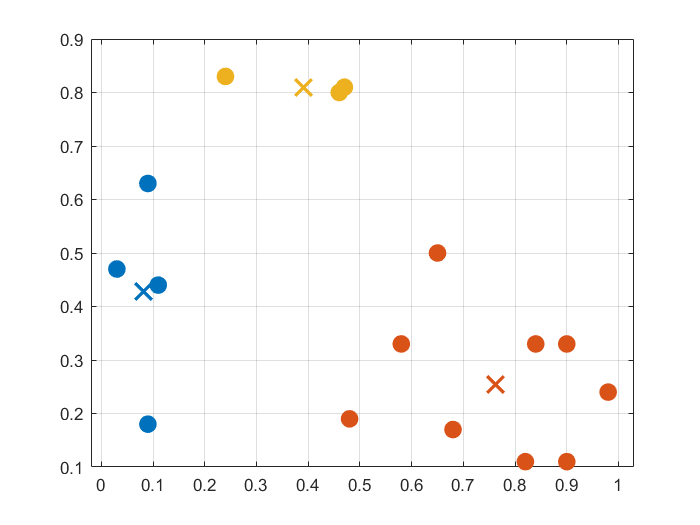
\includegraphics[width=\textwidth]{IMG/R11.png}
		\caption{Euclidiana con M = 1.3}
		\label{fig:r1}
	\end{subfigure}\hfill
	\begin{subfigure}[b]{0.50\textwidth}
		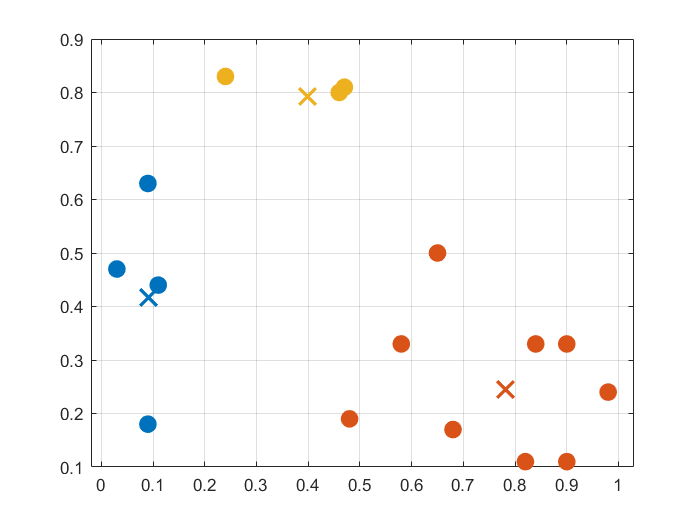
\includegraphics[width=\textwidth]{IMG/R12.png}
		\caption{Euclidiana con  M = 1.6}
		\label{fig:r2}
	\end{subfigure}
	\vspace{\baselineskip} % Espacio vertical entre filas
	\begin{subfigure}[b]{0.50\textwidth}
		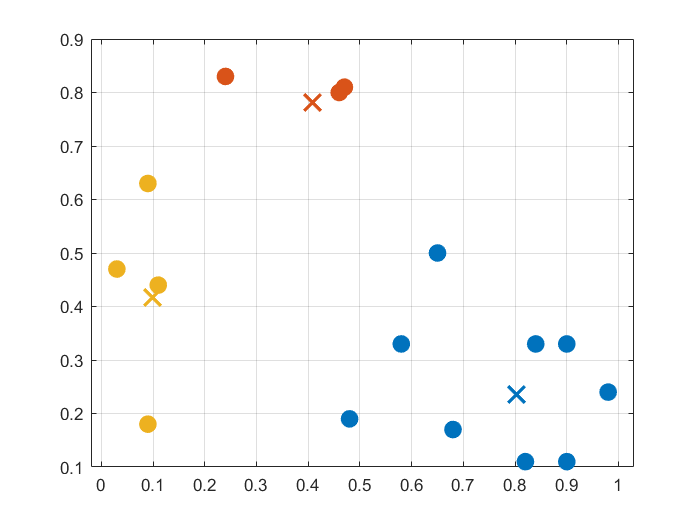
\includegraphics[width=\textwidth]{IMG/R13.png}
		\caption{Euclidiana con  M = 1.9}
		\label{fig:r3}
	\end{subfigure}\hfill
	\caption{Resumen de los resultados con distancia Euclidiana}
	\label{fig:cuadro_r}
\end{figure}

\newpage

\subsection{Resultados para la distancia de Mahalanobis}

\begin{figure}[h!]
	\centering
	\begin{subfigure}[b]{0.50\textwidth}
		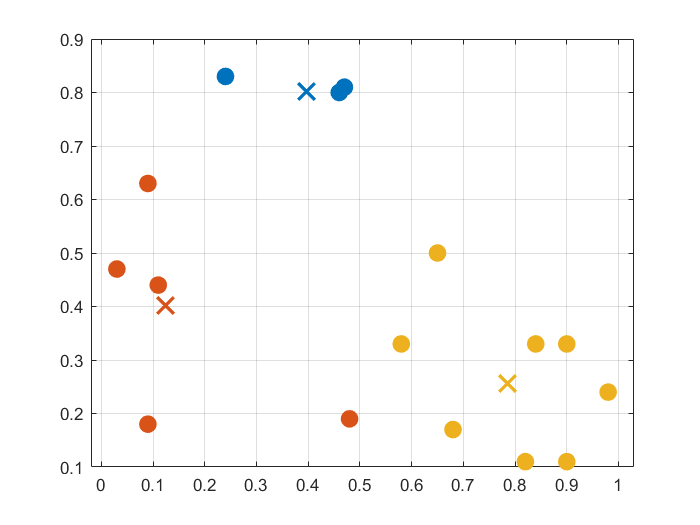
\includegraphics[width=\textwidth]{IMG/R21.png}
		\caption{Mahalanobis con M = 1.3}
		\label{fig:r4}
	\end{subfigure}\hfill
	\begin{subfigure}[b]{0.50\textwidth}
		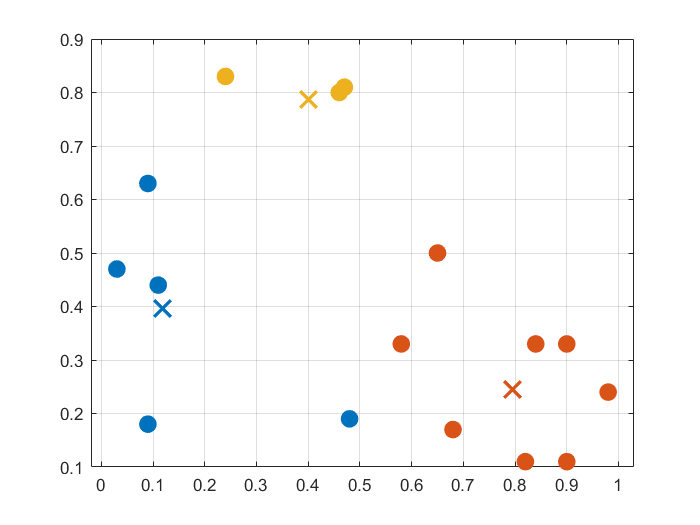
\includegraphics[width=\textwidth]{IMG/R22.png}
		\caption{Mahalanobis con  M = 1.6}
		\label{fig:r5}
	\end{subfigure}
	\vspace{\baselineskip} % Espacio vertical entre filas
	\begin{subfigure}[b]{0.50\textwidth}
		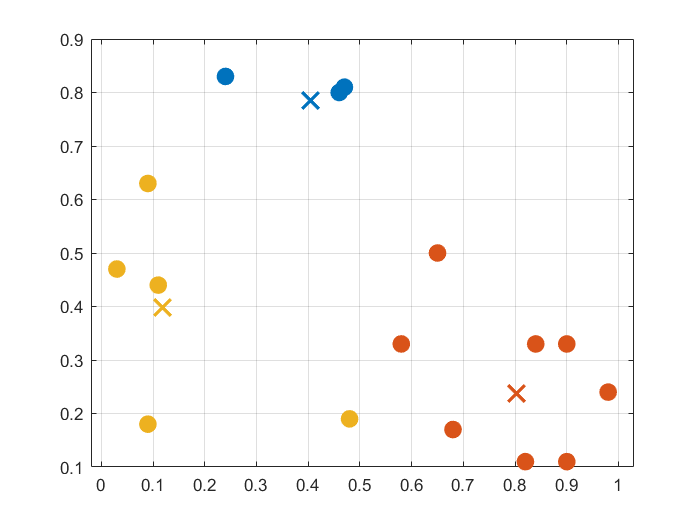
\includegraphics[width=\textwidth]{IMG/R23.png}
		\caption{Mahalanobis con  M = 1.9}
		\label{fig:r6}
	\end{subfigure}\hfill
	\caption{Resumen de los resultados con distancia Mahalanobis}
	\label{fig:cuadro_r2}
\end{figure}


\newpage

\subsection{Resultados para la distancia de Manhattan}

\begin{figure}[h!]
	\centering
	\begin{subfigure}[b]{0.50\textwidth}
		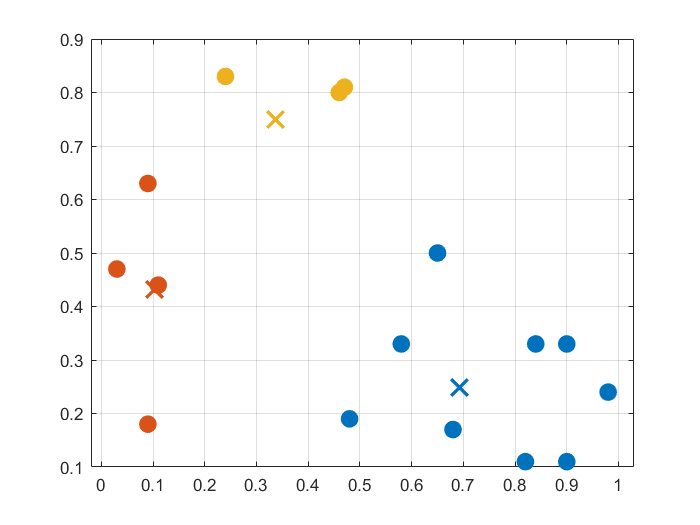
\includegraphics[width=\textwidth]{IMG/R31.png}
		\caption{Manhattan con M = 1.3}
		\label{fig:r7}
	\end{subfigure}\hfill
	\begin{subfigure}[b]{0.50\textwidth}
		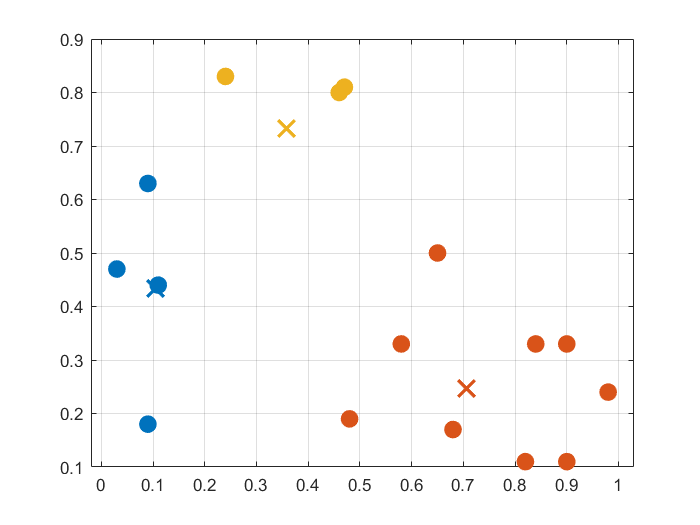
\includegraphics[width=\textwidth]{IMG/R32.png}
		\caption{Manhattan con  M = 1.6}
		\label{fig:r8}
	\end{subfigure}
	\vspace{\baselineskip} % Espacio vertical entre filas
	\begin{subfigure}[b]{0.50\textwidth}
		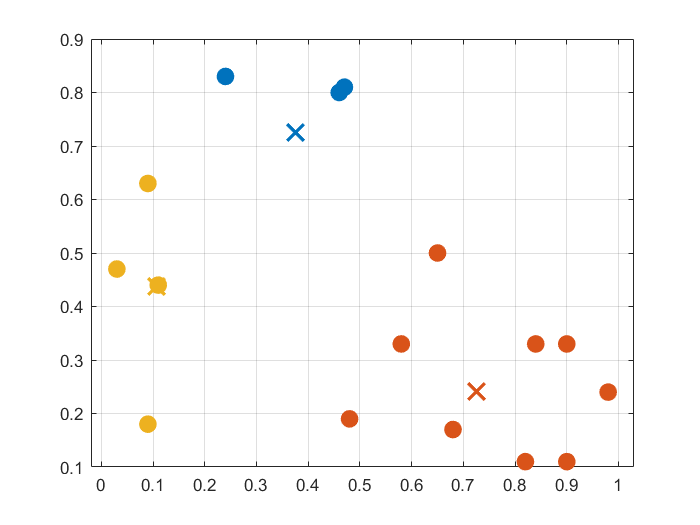
\includegraphics[width=\textwidth]{IMG/R33.png}
		\caption{Manhattan con  M = 1.9}
		\label{fig:r9}
	\end{subfigure}\hfill
	\caption{Resumen de los resultados con distancia Manhattan}
	\label{fig:cuadro_r3}
\end{figure}

\newpage

\section{Conclusiones}

Se observa que el algoritmo logra detectar agrupaciones que se encuentran relativamente "visibiles", siendo que en para las 3 distancias, no hay diferencias internas al variar el parametro de fuzzy $M$. Tambien se encontro que la distancia Euclidiana y la distancia de Manhattan dan los mismos resultados, siendo que la distancia de Mahalanobis  detecta que un punto que las demas distancias identifican cerca del centroide que se encuentra abajo a la derecha, realmente pertenece a el centroide de la izquierda, esto se puede explicar porque la distancia de Mahalanobis pondera en función de las varianzas y covarianzas.

Queda como trabajo futuro realizar la comparativa del desempeño de este algoritmo contra el algoritmo de K-medias clásico.


\newpage

\section{Referencias}

\bibliographystyle{apalike}  % Estilo de cita, puedes cambiarlo si lo prefieres.
\bibliography{Biblio}         % Aquí incluyes el archivo .bib (sin extensión).

\newpage

\section{Anexos}

Este reporte se envía con los códigos anexos que corresponden a:

\begin{enumerate}
	\item El codigo en MATLAB del fuzzy cmeans con las pruebas
	\item El archivo de excel donde se almacenaron los datos.

\end{enumerate}



\end{document}

